\documentclass[12pt]{article}
\usepackage{polski}
\usepackage[utf8]{inputenc}
\usepackage[T1]{fontenc}
\usepackage{amsmath}
\usepackage{amsfonts}
\usepackage{fancyhdr}
\usepackage{lastpage}
\usepackage{multirow}
\usepackage{amssymb}
\usepackage{amsthm}
\usepackage{textcomp}
\frenchspacing
\usepackage{fullpage}
\setlength{\headsep}{30pt}
\setlength{\headheight}{12pt}
%\setlength{\voffset}{-30pt}
%\setlength{\textheight}{730pt}
\pagestyle{myheadings}

\usepackage{tikz}
%\usepackage{tikz-cd}
\usetikzlibrary{arrows}

\newcommand{\bigslant}[2]{{\left.\raisebox{.2em}{$#1$}\middle/\raisebox{-.2em}{$#2$}\right.}}

\newcommand{\mf}[1]{{\mathfrak{#1}}}
\newcommand{\mb}[1]{{\mathbb{#1}}}
\newcommand{\mc}[1]{{\mathcal{#1}}}
\newcommand{\mr}[1]{{\mathrm{#1}}}
\newcommand{\Grass}{{\mathrm{Grass}}}
\newcommand{\Stief}{{\mathrm{Stief}}}

\newcounter{punkt}

\theoremstyle{plain}
\newtheorem{twierdzenie}[punkt]{Twierdzenie}
\newtheorem{twierdzeniebd}[punkt]{Twierdzenie (bez dowodu)}
\newtheorem{lemat}[punkt]{Lemat}

\theoremstyle{definition}
\newtheorem{definicja}[punkt]{Definicja}
\newtheorem{stwierdzenie}[punkt]{Stwierdzenie}
\newtheorem{stwierdzeniebd}[punkt]{Stwierdzenie (bez dowodu)}
\newtheorem{wniosek}[punkt]{Wniosek}

\theoremstyle{remark}
\newtheorem{uwaga}[punkt]{Uwaga}
\newtheorem{przyklad}[punkt]{Przykład}
\newtheorem{cytat}[punkt]{Cytat}


\markright{Piotr Suwara\hfill Topologia działania torusa: 23 października 2012 \hfill}
 
\begin{document}
 \begin{twierdzenie}
  $G= GL_n(\mb{C})$ lub $G=U(n)$, wtedy przestrzeń klasyfikująca $BG=\Grass_n(\mb{C}^\infty) = \bigcup_N \Grass_n(\mb{C}^N)$.
  
  Uniwersalna wiązka dla $U(n)$ to $\Stief_n^{ort}(\mb{C}^n)$ okłady ortonormalne, dla $GL_n(\mb{C})$ to $\Stief_n(\mb{C}^\infty)$ układy liniowo niezależne.
 \end{twierdzenie}
 
 \begin{wniosek}
  $G\subset GL_n(\mb{C})$ domknięta (czyli Lie), wtedy $BG$ ma model będący wstępującą sumą rozmaitości (bo $\Stief_n(\mb{C}^N)/G$ to rozmaitość).
 \end{wniosek}
 
 \begin{wniosek}
  $G \subset GL_n(\mb{C})$ algebraiczna, to $BG$ ma model będący wstępującą sumą rozmaitości algebraicznych.
 \end{wniosek}
 
 \begin{przyklad}
  Niech $G=T=(\mb{C}^\ast)^n$.
 
  $B \mb{C}^\ast = \mb{P}^\infty$.
  
  $B(G \times H) = BG \times BH$, czyli $B(\mb{C}^\ast)^n = (\mb{P}^\infty)^n$.
  
  Z innej strony $ET=\Stief_n(\mb{C}^\infty)$, $BT=\Stief_n(\mb{C}^\infty)/T=\Grass_n^{split}(\mb{C}^\infty) = \{ V \in \Grass_n(\mb{C}^\infty)\text{ wraz z rozkładem } V = L_1 \oplus L_2 \oplus \ldots \oplus L_n\} \to \Grass_n(\mb{C}^\infty)$.
 \end{przyklad}
 
 \begin{przyklad}
  $BSL_n(\mb{C}) = \Stief_n(\mb{C}^\infty)/SL_n(\mb{C}) = \{ V \in \Grass_n(\mb{C}^\infty)\text{ wraz z izomorfizmem }\varphi: \bigwedge^n V \to \mb{C} \} \to \Grass_n(\mb{C}^\infty)$
 \end{przyklad}
 
 \begin{przyklad}
  $BSO_n(\mb{C}) = \{ V \in \Grass_n(\mb{C}^\infty)\text{ wraz z niezdegenerowaną formą kwadratową na }V\}$
 \end{przyklad}
 
 \begin{przyklad}
  Niech $G$ będzie grupą Borela, tj. macierzami górnotrójkątnymi, wtedy $BG = \{ V \in \Grass_n(\mb{C}^\infty)\text{ wraz z filtracją }V_1 \subset \ldots \subset V_n = V\}$, czyli jest to tzw. częściowa rozmaitość flag.
 \end{przyklad}
 
 \begin{twierdzenie}
  Jeśli $G \hookrightarrow H \overset{\pi}{\twoheadrightarrow} K$ ciąg dokładny grup, $G$ normalna, to istnieje rozwłóknienie $BG \to BH \to BK$.
 \end{twierdzenie}
 
 \begin{uwaga}
  $G$ Lie zawiera torus, to $BG$ nie może być skończenie wymiarowe.
 \end{uwaga}
 
 \begin{twierdzeniebd}
  $G$ spójna Lie, $T$ maksymalny torus w $G$, $H^\ast(BG, \mb{Q}) = H^\ast(BT,\mb{Q})^W$, $W=NT/T$.
 \end{twierdzeniebd}
 \pagebreak
 {\bf Kohomologie ekwiwariantne}
 
 Chcemy je tak zdefiniować, by $G$-ekwiwariantna homotopijna równoważność $X \to Y$ indukowała izomorfizm na ekwiwariantnych kohomologiach.
 
 \begin{definicja}
  $H_G^\ast(X) = H^\ast(EG \times_G X)$
 \end{definicja}
 
 \begin{uwaga}
  $H^\ast_{\underline{G}}(\underline{X})$ jest funktorem kontrawariantnym ze względu na $X$ oraz kontrawariantnym ze względu na $G$.
 \end{uwaga}
 
 \begin{twierdzenie}
  $f:X \to Y$, $G$-ekwiwariantna homotopijna równoważność indukuje izomorfizm $H_G^\ast(Y) \simeq H_G^\ast(X)$.
 \end{twierdzenie}
 
 \begin{uwaga}
  $H_G^\ast(X)$ jest algebrą nad $H^\ast(BG)$.
 \end{uwaga}
 
 \begin{uwaga}\raisebox{-0.7\height}{
  \begin{tikzpicture}
   \node (X) at (0,1) {$X$};
   \node (EGX) at (2,1) {$EG \times_G X$};
   \node (XG) at (4,1) {$X/G$};
   \node (BG) at (2,0) {$BG$};
   \path[->,>=angle 90] (EGX) edge (BG);
   \path[right hook->,>=angle 90] (X) edge (EGX);
   \path[->>,>=angle 90] (EGX) edge (XG);
  \end{tikzpicture}}
  indukuje ciąg homomorfizmów \raisebox{-0.6\height}{
  \begin{tikzpicture}
   \node (XG) at (0,0) {$H^\ast(X/G)$};
   \node (GX) at (2,0) {$H_G^\ast(X)$};
   \node (X) at (4,0) {$H^\ast(X)$};
   \path[->,>=angle 90]
   (XG) edge (GX)
   edge [bend right] node[above]{$\pi^\ast$} (X)
   (GX) edge (X);
   
  \end{tikzpicture}}
 \end{uwaga}
 
 \begin{twierdzenie}
  Jeśli $G$ działa wolno na $X$, to $H^\ast(X/G) \to H^\ast(X)$ izomorfizm.
 \end{twierdzenie}
 
 \begin{lemat}
  $G$ działa wolno, to włókna są ściągalne, czyli $EG \times_G X \simeq_{htp} X/G$.
 \end{lemat}
 
 \begin{stwierdzenie}
  Jeśli $X'$ wolna $G$-przestrzeń, $X' \to X$ to $G$-ekwiwariantna homotopijna równoważność, to $H_G^\ast(X) = H^\ast(X'/G)$.
 \end{stwierdzenie}















\end{document}
 
 
